%
% CryptoWars (TM)
%

\dropcap{U}{ndoubtedly}, quantum technologies will be most impactful (and disruptive!) in the area of information security, something of fundamental importance to us all on a daily basis, vital to the world economy. Quantum technologies will be important both in terms of breaking and maintaining security, with the former mandating interest in the latter.

In Sec.~\ref{sec:homo_blind} we discussed encrypted outsourced quantum computation as an important concept in future cloud quantum computing. In this section we will step back from full-fledged distributed quantum computation, instead focussing on more elementary protocols for simple secure communication.

Today, the ability to communicate secretly with others is completely taken for granted in all but a few nations and resides in every smartphone and desktop PC. Furthermore, the encryption technologies available to the average consumer are extremely strong, the same as those used by large organisations, including world governments.

%
% What is Security?
%

\section{What is security?}\index{Computational security}\index{Information-theoretic security}\label{sec:comp_vs_inf_th_sec}

\dropcap{B}{efore} describing any specific cryptographic protocols, let us define what is meant by `security' in a cryptographic context. We differentiate between \textit{information theoretic security}\index{Information-theoretic security}, as opposed to \textit{computational security}\index{Computational security}:

\begin{itemize}
	\item Information-theoretic security: the laws of quantum information bound the amount of information that can be extracted from a system, irrespective of measurement or computational operations. Thus, such security can be regarded as attack-independent.
	\item Computational security: is based on the assumption that an adversary's computational resources are insufficient to perform cryptanalysis or brute-force cracking. Clearly the former makes a far stronger statement about the security of a protocol than the latter.
\end{itemize}

Classical public- and private-key encryption protocols are typically based upon the assumption of computational security (e.g the computational complexity of performing integer factorisation in the case of RSA public-key encryption, or solving a complex satisfiability problem in the case of private-key encryption), whereas quantum encryption protocols are typically information theoretically secure (e.g the one-time pad using QKD).

%
% Classical Cryptography
%

\section{Classical cryptography}\index{Classical cryptography}

\dropcap{W}{e} begin with an introduction into \textit{classical} cryptography, so as to understand its limitations, which logically leads us into how quantum mechanics can assist in overcoming these limitations. We only scratch the surface of these extremely well-researched field, reviewing some of the most important and widely used protocols. For a deeper understanding of classical cryptography we refer the interested reader to \cite{bib:Schneier96}.

%
% Private-Key Cryptography
%

\subsection{Private-key cryptography}\index{Private-key cryptography}

Private- (or symmetric-) key cryptography is perhaps the most basic (and useful) cryptographic primitive, enabling encryption of a channel between two parties who share a secret key\index{Private key} -- a random bit-string of length determined by the encryption algorithm. The same secret key is employed for both encryption and decryption operations, making it of utmost importance that it be retained secret.

Private key cryptography has a long history, in fact going back to ancient times, enabling the secret sharing of diplomatic messages between emperors and empires, e.g the so-called \textit{Caesar cipher}\index{Caesar cipher}, a simple substitution cipher\index{Substitution cipher} based on shifting the letters of the alphabet. However it was a niche technology that very few utilised, since it had to be implemented by hand without computers.

Today there are countless freely available private-key cryptographic protocols available online, and some have been standardised by standards institutes. Currently, the Advanced Encryption Standard (AES)\index{Advanced Encryption Standard (AES)} is a standard endorsed by the US government, replacing the earlier standardised Data Encryption Standard (DES)\index{Data Encryption Standard (DES)} whose mere 56-bit key-length is today considered insecure. AES is a block cipher\index{Block cipher}, meaning that it divides data into small blocks of 128 bits, each of which are encrypted independently, and operates with key lengths of up to 256 bits (referred to as AES256), making it very robust against (even quantum) brute-force attacks (Sec.~\ref{sec:attacks_on_class}). The length of the plaintext and ciphertext is the same, meaning there is no bandwidth overhead when communicating encrypted data across a network.

%
% One-Time Pad Cipher
%

\subsection{One-time pad cipher}\index{One-time pad}

There is one and only one \textit{provably} secure (in the sense of information-theoretic security\index{Information-theoretic security} as opposed to computational security\index{Computational security}) encryption protocol -- the \textit{one-time pad}\index{One-time pad}. This protocol requires Alice and Bob to share a random secret key as long as the message (plaintext\index{Plaintext}) being communicated between them. The two bit-strings undergo bit-wise XOR operations to form the ciphertext\index{Ciphertext}. Mathematically,\index{One-time pad}
\begin{align}
c = s \oplus k,
\end{align}
where $\oplus$ is the bitwise XOR operation (equivalently addition modulo 2), and $c$, $s$ and $k$ are the ciphertext, plaintext and key bit-strings respectively, all of which are of the same length,
\begin{align}
	|c|=|s|=|k|.
\end{align}

The security of this protocol is easy to see intuitively -- with an appropriate choice of key, \textit{any} plaintext of the same length could be inferred from the ciphertext. This means that there is no possibility of performing any kind of frequency analysis\index{Frequency analysis}, as the ciphertext string has maximum entropy\index{Entropy} (inherited from the maximum entropy of the key, and assuming a strong cryptographic random bit generator) and thus no correlations. Since every possible valid plaintext can be recovered using an appropriate key, a cracking algorithm is unable to find a unique plaintext matching the ciphertext, since all are equally valid decryptions.

Importantly, the secrecy of the one-time pad\index{One-time pad} strictly requires that a key never be reused. A fresh key must be generated for each message sent, otherwise trivial frequency analysis\index{Frequency analysis} techniques can be employed to compromise security. If the same key $k$ is used to encode two messages $s_1$ and $s_2$, yielding ciphertexts,
\begin{align}
c_1&=s_1\oplus k,\nonumber\\
c_2&=s_2\oplus k,
\end{align}
then we trivially obtain,
\begin{align}
c_1 \oplus c_2 &= (s_1 \oplus k) \oplus (s_2 \oplus k) \nonumber \\
&= (s_1 \oplus s_2) \oplus (k \oplus k) \nonumber \\
&= s_1 \oplus s_2,
\end{align}
which is independent of the key. Now a frequency analysis on the bitwise XOR of two plaintexts can be applied, without requiring any knowledge of the key whatsoever.

Needless to say, the requirement for keys of the same length as the plaintexts, which cannot be reused, raises the obvious criticism that now secret key-sharing is as difficult as sharing a secret message in the first place. This reduces the problem of perfect secrecy of arbitrary messages to the secrecy of shared randomness. 

Although during the Cold War Soviet diplomats would literally carry briefcases between countries full of paper with random data for use in a one-time pad, it is clearly not suitable for everyday applications!

%
% Public-Key Cryptography
%

\subsection{Public-key cryptography}\index{Public-key cryptography}

While private-key cryptography solves the problem of end-to-end cryptography, it has one main downfall -- how does one share a private key between two parties? After all, if we had the ability to secretly share keys between ourselves, wouldn't we just use that method to directly communicate, bypassing the unnecessary cryptographic protocol?

Public- (or asymmetric-) key cryptography addresses this issue by replacing the private key with two keys (known as a key-pair\index{Key-pair}), one used solely for \textit{encryption}, the other solely for \textit{decryption}. Importantly, these two keys are non-trivially related and cannot be efficiently computed from one another. To send a message to a friend I can send him my encryption (public) key that he is only able to use for preparing an encrypted message for me. No security is required when sharing the public key since an eavesdropper can't use it for decryption. Finally, I am able to decrypt the message using my decryption (private) key, which I kept completely to myself and never shared with anyone.

RSA \cite{bib:RSA} was the first published public-key cryptographic protocol, and forms the backbone for most encryption used on the internet today. It achieves its security based on the belief that factorising large integers into constituent primes is a computationally hard problem -- a so-called `trapdoor function'\index{One-way functions}. The algorithm is built upon number theory using modular arithmetic, described in detail in Alg.~\ref{alg:RSA}.

\begin{table}[!htbp]
\begin{mdframed}[innertopmargin=3pt, innerbottommargin=3pt, nobreak]
\texttt{
function RSAGenerateKey():
\begin{enumerate}
\item $p$ = randomPrime()
\item $q$ = randomPrime()
\item if($p=q$) goto 1
\item $n = pq$
\item $\lambda = \mathrm{lcm}(p-1,q-1)$
\item $e = \mathrm{coprime}(\lambda) \,\,\mathrm{s.t} \,\,e<\lambda$
\item $d = e^{-1}\,(\mathrm{mod} \, \lambda)$
\item publicKey = $\{n,e\}$
\item privateKey = $\{n,d\}$
\item keyPair = \{publicKey,privateKey\}
\item return(keyPair)
\item $\Box$	
\end{enumerate}
function RSAEncrypt(plaintext, publicKey):
\begin{enumerate}
\item $\mathtt{cipertext} = \mathtt{plaintext}^e \, (\mathrm{mod} \, n$)
\item return(ciphertext)
\item $\Box$
\end{enumerate}
function RSADecrypt(ciphertext, privateKey):
\begin{enumerate}
\item $\mathtt{plaintext} = \mathtt{ciphertext}^d \, (\mathrm{mod} \, n)$
\item return(plaintext)
\item $\Box$
\end{enumerate}
}
\end{mdframed}
\captionspacealg \caption{Number-theoretic algorithms based on modular arithmetic for RSA key generation, encryption and decryption.} \label{alg:RSA}
\end{table}

Since RSA, numerous other public-key cryptosystems have been developed, based on different choices of trapdoor function. Most notably, elliptic curve cryptography\index{Elliptic curve cryptography} has gained much attention. However, RSA remains the most widely used and well studied public-key cipher.

To mitigate the need for constant one-on-one exchange of public-keys, many key servers\index{Key servers} exist around the globe, which maintain databases of people's public-keys. These servers are in a position of trust, vouching for the identities associated with their stored public-keys.

%
% Key Exchange Protocols
%

\subsection{Key exchange protocols}

A downside of RSA is that ciphertexts are in general much longer than plaintexts, unlike private-key protocols where the ciphertext is always the same length as the plaintext. For this reason it is typically not used to directly encrypt long messages, since the memory and bandwidth overheads would be undesirable. Instead, RSA is typically employed in conjunction with private-key cryptography in a key exchange protocol\index{Key exchange protocol}. Here the public-key system communicates a private \textit{session key}\index{Session key} between parties, which is subsequently employed in a private-key protocol, without incurring the time and memory overhead that RSA does. In Sec.~\ref{sec:brute_force_attacks} we point out that quantum computers are not believed to be able to efficiently crack private-key protocols, but instead effectively reduce their key length by a factor of 1/2, which is easily counteracted to restore security.

Numerous key exchange protocols have been formulated, the best known being the Diffie-Hellman\index{Diffie-Hellman protocol} protocol \cite{DiffieHellman}, which has been widely adopted on the internet.

%
% Digital Signatures
%

\subsection{Digital signatures} \label{sec:dig_sig} \index{Digital signatures}

Rather than cryptographically ensuring the secrecy of messages, a user may wish to prove their identity when sending a message, such that the recipient can be certain it originated from who it says it does, and accurately conveys what they said. This is achieved using \textit{digital signatures}.

Digital signatures can be easily implemented using the RSA protocol\index{RSA protocol}, but swapping the role of the public and private keys. Now the public key can only be used for decrypting a message, and the private key can only be used for encrypting it. As before, it is computationally hard to infer one from the other. The protocol for sending and verifying a digitally signed message is shown in Alg.~\ref{alg:dig_sig}.

\begin{table}[!htbp]
\begin{mdframed}[innertopmargin=3pt, innerbottommargin=3pt, nobreak]
\texttt{
function DigitalSignature(message,keyPair):
\begin{enumerate}
\item Alice prepares a short \textit{digest}\index{Digest} of her message using a cryptographic hash function\index{Hash functions}, such as SHA256\index{SHA256} (Sec.~\ref{sec:hashing}),\\
	\vspace{1mm} 
	$digest=SHA256(message)$
	\item Alice encrypts the digest using her private key. This forms the `digital signature',\\
	\vspace{1mm} 
	$signature = RSAEncrypt(digest,privateKey)$
	\item Alice transmits the digital signature and original message to Bob,\\
	\vspace{1mm} 
	$signedMessage = \{message,signature\}$
	\item Bob hashes the received message,\\
	\vspace{1mm} 	
	$hash=SHA256(message)$
	\item Bob uses Alice's public-key to decrypt her digital signature,\\
	\vspace{1mm} 
	$decryptedHash =$\\
	$RSADecrypt(signature,publicKey)$
	\item Bob compares his calculated hash with Alice's decrypted hash for consistency. If the two hashes are identical, Bob concludes the message was authentic,\\
	\vspace{1mm} 
	$if(decryptedHash=hash)$\\
	$\,\,return(pass)$\\
	$else$\\
	$\,\,return(fail)$
	\item $\Box$
\end{enumerate}
}
\end{mdframed}
\captionspacealg \caption{Protocol for digitally signing a message using public-key cryptography (RSA) and a cryptographic hash function (SHA256).} \label{alg:dig_sig}
\end{table}

The key point from the security perspective is that the private key cannot be efficiently inferred from the public key. So although everyone has access to Alice's public key, no one is able to counterfeit messages since they cannot create encrypted signatures without access to her private key -- signatures can be easily verified but not created.

Because this protocol is implemented using ordinary RSA\index{RSA protocol}, albeit with reversed roles for the key-pair, it shares the same security strengths and vulnerabilities as RSA public-key cryptography (Sec.~\ref{sec:attacks_on_class}).

Like RSA cryptography, key servers\index{Key servers} exist, maintaining databases of people's public-keys and their associated identities.

Because RSA-encrypted messages are long, digital signature protocols do not sign the full document directly. Instead they create a message digest\index{Message digests} of the document using a cryptographic hash function, which is signed using RSA. These hash functions have the property that they cannot for forged or manipulated, providing an accurate summary of a document, but with extremely low memory overhead (256 bits is typical). Hash functions are discussed next in Sec.~\ref{sec:hashing}.

%
% Hashing
%

\subsection{Hashing} \label{sec:hashing} \index{Hash functions}

Hash functions are functions that map a long string of arbitrary length to a short, fixed-size string with quasi-random behaviour,
\begin{align}
	f_\mathrm{hash}:\,\{0,1\}^n \to \{0,1\}^m,
\end{align}
for an $n$-bit input and $m$-bit output hash, where $n$ is variable and $m$ is fixed. They are an example of `one-way functions'\index{One-way functions} that are computationally easy to compute in the forward direction, but extremely hard to invert. That is, given a hash, it is computationally difficult to find input strings that map to that value.

Hash functions have broad applicability throughout computer science, but here we are most interested in \textit{cryptographic hash functions} for use in cryptography, which impose strong conditions on the difficulty of inversion and their quasi-random characteristics. Most notably, changing a single bit in the input string ought to flip approximately half the bits of the hash on average.

The standard cryptographic hash function with mainstream adoption is the 256-bit Secure Hashing Algorithm (SHA256\index{SHA256}), which generates 256-bit hashes. The algorithm is extremely efficient to implement digitally, and exhibits $O(n)$ runtime for input string length $n$.

Cryptographically, hash functions are useful for creating message digests\index{Message digests}, which act as a highly condensed checksum\index{Checksum} of a document that can be utilised as a digital signature (Sec.~\ref{sec:dig_sig}).

Note that because the function in general maps longer strings to shorter ones, there are necessarily \textit{collisions}\index{Hash collisions} -- multiple inputs for a given output. However, for strong cryptographic hash functions their behaviour is sufficiently random that two distinct messages will almost certainly yield completely different hashes (even if the messages are very similar), making it all but impossible for someone to make the claim that Alice said something she did not. This property is extremely important for the security of digital signatures.

%
% Attacks On Classical Cryptography
%

\section{Attacks on classical cryptography}\index{Cryptographic attacks}\label{sec:attacks_on_class}

\dropcap{H}aving introduced the main classes of classical cryptographic protocols, we now turn our attention to their weaknesses and vulnerabilities, both against adversaries with classical or quantum computational resources.

%
% Classical Attacks
%

\subsection{Classical attacks}

All known classical attacks against any respected classical cryptosystem involve tremendous computational resources. After all, were this not the case the cryptosystem would be considered weak and would never have become widely adopted in the first place!

%
% Brute-Force
%

\subsubsection{Brute-force}\index{Brute-force attacks}\label{sec:brute_force_attack}

The most obvious approach to cracking a cryptosystem is to systematically try out all possible keys until we find one that correctly decodes the encrypted message. This is also the most na\"ive approach, and one which is computationally intractable for real-world key lengths. Specifically, for a key length of $k$ bits (\mbox{$k=256$} for AES256), there are $2^k$ possible keys to try, and on average we will wait for $2^{k-1}$ trials before choosing the right one. Clearly an average waiting time of $2^{255}$ is not plausible!

%
% Cryptanalysis
%

\subsubsection{Cryptanalysis}\index{Cryptanalysis}

Far better than waiting the age of the universe for the right key to turn up, is \textit{cryptanalysis}. Here we study patterns between input and output strings from a cipher utilising a particular key. There are many variations on this, but include techniques such as \cite{bib:Schneier96}:

\begin{itemize}
	\item Known plaintext attacks (KPA)\index{Known plaintext attack}: Through alternate means of espionage, the attacker is able to possess \textit{both} a ciphertext and its associated plaintext. Knowing both the input and output to the encryption algorithm may then reveal information about the key relating them. This technique was important to Alan Turing's successful cracking of the German Enigma\index{Enigma machines} encryption protocol during World War II.
	\item Chosen plaintext attack (CPA)\index{Chosen plaintext attack}: The same as a KPA except that the adversary has the ability to choose what the known plaintext is.
	\item Linear cryptanalysis\index{Linear cryptanalysis}: A technique for representing ciphers as linear systems, to which KPA are applied.
	\item Differential cryptanalysis\index{Differential cryptanalysis}: We analyse how changes in input bits propagate through the cipher to modulate output bits. Typically this type of technique operates as a CPA.
\end{itemize}
 
%
% Integer Factorisation
%
 
\subsubsection{Integer factorisation}\index{Integer factorisation}

In the case of RSA encryption, whose security derives from the believed computational hardness of factorising large numbers, the most efficient known classical algorithm for integer factorisation is the general number field sieve (GNFS)\index{General number field sieve}, with time-complexity,
\begin{align} \label{eq:GNFS_scaling}
	O(\exp (O(1) (\log n)^{\frac{1}{3}} (\log\log n)^{\frac{2}{3}})),
\end{align}
which scales poorly for large $n$, keeping in mind that present-day implementations of RSA accommodate key lengths of up to 4,096 bits, as for example is implemented by the Pretty Good Privacy (PGP)\index{Pretty Good Privacy (PGP)} package.

%
% Quantum Attackes
%

\subsection{Quantum attacks}

Having established that classical attacks against strong classical cryptosystems are quite limited by their implausible computational requirements, what if our adversary now has quantum computational resources? Does this change the game?

%
% Brute-Force
%

\subsubsection{Brute-force}\index{Brute-force}\label{sec:brute_force_attacks}

A brute-force attack by a quantum computer does not offer us the exponential improvement attacker Eve might hope for. However, we can gain a quadratic improvement by cleverly exploiting Grover's search algorithm (Sec.~\ref{sec:quantum_algs})\index{Grover's algorithm}.

To do this, we treat the brute-force cracking algorithm as a satisfiability problem, similar to how Grover's is employed to enhance \textbf{NP}-complete problems. Specifically, our oracle implements the code's decryption operation, taking as input a qubit string representing the key. After decoding the message with the key, the oracle runs an appropriate test on the decrypted message to determine whether it is a legitimate decoded message. For example, it could run an English language test -- a message decoded incorrectly with the wrong key will appear very random and almost certainly won't pass such a test. The oracle tags an element passing this test, which the Grover algorithm searches for, yielding the associated key.

Note that when performing a brute-force attack against a private encryption key\index{Private-key cryptography}, a quadratic speedup effectively halves the key length in terms of algorithmic runtime, since \mbox{$O(\sqrt{2^k}) = O(2^{k/2})$}. Thus, in the quantum era private key lengths will need to be doubled to maintain the same security against brute-force attacks.

This same technique of treating encryption as an oracle within a quantum search algorithm can be utilised to invert hash functions\index{Hash functions}. However, in this case there will necessarily be multiple solutions.

%
% Cryptanalysis
%

\subsubsection{Cryptanalysis}\index{Cryptanalysis}

In the case of private-key cryptosystems such as AES\index{Advanced Encryption Standard (AES)}, no quantum-enhanced cryptanalytic techniques have been described, which offer an exponential enhancement. Thus, modulo doubling key-lengths to counter a Grover attack, these cryptosystems are not regarded as being compromised by quantum computing.

%
% Integer Factorisation
%

\subsubsection{Integer factorisation}\index{Integer factorisation}

In the case of RSA public-key cryptography the attack is more direct -- with access to a scalable quantum computer, Shor's algorithm\index{Shor's algorithm} can be employed to efficiently factorise large integers, allowing private keys to be retrieved from public keys. Unlike the brute-force attacks, which yielded only a quadratic enhancement, Shor's algorithm is exponentially faster than the classical GNFS, requiring runtime of only,
\begin{align}
	O((\log n)^2(\log\log n)(\log\log\log n)).
\end{align}
Compare this with the classical case given in Eq.~(\ref{eq:GNFS_scaling}).

%
% Bitcoin & The Blockchain
%

\section{Bitcoin \& the Blockchain}\index{Blockchain}\index{Bitcoin}\label{sec:bitcoin_blockchain}

\dropcap{O}{ne} of the most exciting new cryptographic applications that has emerged in recent years is the Blockchain, a secure distributed ledger\index{Distributed ledger} for recording the execution of contracts and transactions. This has enabled cryptocurrencies\index{Cryptocurrencies}, most notably Bitcoin, to emerge as a secure digital alternative to conventional fiat currencies.

More recent developments, such as the Ethereum project\index{Ethereum}, develop the distributed ledger further to allow executable code to be committed to the Blockchain, opening the prospects for self-enforcement and -execution of completely arbitrary contracts, a potential game-changer for the operation of financial and derivative markets.

In the Blockchain protocol, the validity of contracts and transactions is recognised collectively by participants using an encrypted digital ledger\index{Ledger}. The ledger records the complete history of all Blockchain transactions, which are digitally signed (Sec.~\ref{sec:hashing}) by network participants using elliptic curve public-key cryptography\index{Digital signatures}\index{Elliptic curve cryptography}. A democratic process ensures that, provided a single user doesn't monopolise the network, recorded transactions are legitimate, recognised collectively. This is secured by network participants digitally signing off on transactions as they take place.

The Bitcoin protocol builds on top of the Blockchain to create a secure digital cryptocurrency. This requires the introduction of another sub-protocol, \textit{mining}\index{Bitcoin mining}, where units of currency (`coins'\index{Coins}) are created. The protocol cryptographically ensures that there is an upper-bound on the number of coins that can exist, thereby preventing forgery and an inflationary blowout in the money supply.

The mining process is based upon the computational hardness of inverting (double) SHA256 hashing\index{Hash functions}\index{SHA256}. A legitimate Bitcoin is defined by a string with a hash satisfying a thoughtfully chosen constraint, specifically one which hashes to a value within some range,
\begin{align}
	\epsilon_\mathrm{lower}\leq \mathrm{SHA256}(\mathrm{SHA256}(x_\mathrm{coin})) \leq \epsilon_\mathrm{upper}.
\end{align}
This is slightly weaker than inverting hash functions, but is nonetheless a task that can only be approached via brute-force hashing in the forward direction. This associates computational complexity with the mining process, and hence computational integrity of the money supply, whilst upper bounding the number of unique coins that can exist. This technique is known as `proof-of-work'\index{Proof-of-work}, for associating something of value with proof that certain amounts of computation were required to achieve it\footnote{In future implementations of Blockchain protocols, the proof-of-work required for a given protocol can be arbitrarily manipulated to accommodate for technological advances in computational power, for example via the adoption of quantum computing. The amount of work required to satisfy the constraint grows as we narrow the range \mbox{$\epsilon_\mathrm{upper}-\epsilon_\mathrm{lower}$}, providing us with much leverage to manipulate the complexity of the proof-of-work, and hence the rate of growth in the money supply, equivalently the rate of inflation\index{Inflation rate}.}. This idea was originally borrowed from the Hashcash protocol\index{Hashcash}, where proof-of-work is employed to associate work (and hence monetary value) with sending emails so as to eliminate automated spamming bots.

The two key algorithms for Bitcoin and the Blockchain are therefore hashing and public-key digital signatures. Both of these are subject to enhanced quantum attacks.

Hashing does not have any known quantum algorithm with exponential improvement, however using a Grover search\index{Grover's algorithm} one can achieve a quadratic speedup, using the same idea as for enhancing \textbf{NP}-complete problems by treating the hash function as a search oracle\index{Oracles}. This however does not pose a fundamental security concern as it will speed up the Bitcoin mining process, but does not circumvent the upper-bound on the number of coins that may be in existence. Already classical mining has pushed the Bitcoin money supply close to its asymptotic maximum and there is limited room for additional mining\footnote{Bitcoin mining has gained so much traction and become so competitive that desktop PCs have become uneconomical for mining. Instead miners are resorting to utilising specialised hardware in the form of CUDA cores\index{CUDA cores}, FPGAs\index{FPGA} and ASICs\index{ASIC} (or by secretly using the company supercomputer while the boss isn't looking).}.

Elliptic curve public-key cryptography, like RSA, has a known efficient quantum attack via Shor's algorithm\index{Shor's algorithm}. In the context of implementing digital signatures this implies that an adversary could fraudulently sign off on illegitimate transactions, thereby committing falsified contracts to the Blockchain.

A detailed investigation into the vulnerability of the Blockchain to quantum attacks was performed by \cite{bib:TomamichelBlockchain}. However, it is near impossible to predict the future rate of growth in quantum computer technology and hence over what kind of timescale the Blockchain will be compromised. But it is certain that a full compromise is inevitable at some point in the future.

To address this security threat, quantum-resistant hashing and public-key cryptographic protocols will need to be developed. In the former case this can easily be achieved by increasing hash lengths so as to offset the quadratic enhancement offered by Grover's algorithm\index{Grover's algorithm}. In the latter case this will require post-quantum public-key cryptosystems (to be discussed in the next section, Sec.~\ref{sec:end_of_class_crypto}).

Evidently, the lifespan of exisiting Blockchain technologies is limited and in the quantum future post-quantum Blockchain algorithms will be required to ensure the survival of cryptocurrencies.

%
% The End Of Classical Cryptography?
%

\section{The end of classical cryptography?} \label{sec:end_of_class_crypto}

\dropcap{T}{he} vulnerability of RSA to attacks by quantum computers raises the question whether this spells the end of classical cryptography and compromises the security of much of the present-day internet.

Thankfully, there are two saving graces. First of all, much research is being carried out into \textit{post-quantum classical cryptography}\index{Post-quantum classical cryptography}. That is, public-key cryptosystems based upon trapdoor functions\index{One-way functions} that reside outside of \textbf{BQP} and are therefore not efficiently attacked by quantum computers. One such line of research is to construct cryptosystems based upon \textbf{NP}-complete problems, such as the McEliece protocol\index{McEliece protocol} \cite{bib:McEliece}. Recall from Fig.~\ref{fig:complexity_classes} that \textbf{NP}-complete is strongly believed to reside completely outside of \textbf{BQP}. However, while many computer scientists might be comfortable with such a level of security, it is nonetheless based on the unproven conjecture that \textbf{NP}-complete and \textbf{BQP} do not intersect, i.e \mbox{$\mathbf{NP}\nsubseteq\mathbf{BQP}$}. What would be much more satisfying would be protocols demonstrating information-theoretic security\index{Information-theoretic security} rather than computational security\index{Computational security}. Here quantum mechanics can help us -- \textit{quantum cryptography}.

%
% Quantum Cryptography
%

\section{Quantum cryptography}\index{Quantum cryptography}

\dropcap{A}s quantum physics can compromise some important aspects of classical cryptography, can it perhaps be similarly exploited to make new cryptosystems that are immune even to quantum adversaries? Thankfully the answer is yes... at least some of the time.

%
% Quantum Key Distribution (QKD)
%

\subsection{Quantum key distribution} \label{sec:QKD} \index{Quantum key distribution (QKD)}

%Aside from quantum computing, a central use for quantum technologies is in cryptography \cite{bib:Gisin02}. The demand for secure cryptography is now extremely important in the context of electronic commerce and general security of information transmission in the internet age. Electronic currencies such as Bitcoin\index{Bitcoin} depend on cryptographic protocols in order to secure the value of assets, assign ownership certificates\index{Owner certificates}, and secure the currency against fraud. However such protocols are based upon the computational complexity of certain mathematical problems (\textit{computational security}\index{Computational security}), and are not fundamentally secure in the presence of limitless computational resources, or quantum computers. Therefore, using quantum mechanical protocols based on physical principles (\textit{information-theoretic security}\index{Information-theoretic security}) rather than computational limitations, are favourable in the sense of future-proofing security.

\comment{Add more advanced protocols? Decoy states, untrusted devices, device independent QKD, etc. etc.}

Quantum key distribution (QKD) protocols facilitate shared, secret randomness, where any intercept-resend\index{Intercept-resend attack} (or man-in-the-middle attack) attack may be detected and rejected, guaranteed by the laws of quantum physics (specifically the Heisenberg uncertainty principle\index{Heisenberg uncertainty principle} and no-cloning theorem\index{No-cloning theorem}). This shared, secret randomness may subsequently be employed in a one-time pad cipher\index{One-time pad}, presenting us with true information-theoretic security\index{Information-theoretic security}.

The central notion to QKD protocols, in their numerous manifestations, is that measurement of quantum states invokes a wavefunction collapse. When measuring a state in a basis for which that state is not an eigenstate, this necessarily changes the state. QKD relies on this simple result from quantum mechanics to reveal any eavesdropper performing an intercept-resend attack\index{Intercept-resend attack} via the changes to transmitted quantum states that this would induce.

QKD is a relatively mature technology with already several commercial systems being available off-the-shelf\footnote{Examples of companies selling off-the-shelf QKD hardware include \href{http://www.magiqtech.com}{MagiQ} and \href{http://www.idquantique.com}{ID Quantique}.} and initial space-based implementations have been successfully demonstrated \cite{Pan}.

It is easy to see the utility of quantum networks in enabling commodity deployment of QKD -- users desire to communicate photons across long-range ad hoc networks, with low loss and dephasing. A global quantum internet would allow quantum cryptography to truly supersede classical cryptography, bypassing the vulnerabilities faced by classical cryptography in the era of quantum computing.

%
% BB84 Protocol
%

\subsubsection{BB84 protocol}\index{BB84 protocol}

The first described QKD scheme was the \textit{BB84} \cite{bib:BennetBrassard84}\index{BB84 protocol} protocol, which exploits the fact that states encoded in the $\hat{Z}$-basis but measured in the $\hat{X}$-basis (and vice versa) collapse randomly, yielding completely random measurement outcomes, whereas states measured in the same basis in which they were encoded always correctly communicate a single bit of information.

Implemented photonically, BB84 requires only the transmission of a sequence of single photons, polarisation-encoded\index{Polarisation encoding} with random data.

The BB84 protocol is described in detail in Alg.~\ref{alg:bb84} in the context of polarisation-encoded photons, which is the most natural (but not only) setting for this protocol. An example evolution of the protocol is illustrated in Fig.~\ref{fig:BB84_example}

\begin{table}[!htbp]
\begin{mdframed}[innertopmargin=3pt, innerbottommargin=3pt, nobreak]
\texttt{
function BB84():
\begin{enumerate}
\item Alice chooses a random bit, $0$ or $1$.
\item Alice randomly chooses a basis, $\hat{X}$ or $\hat{Z}$.
\item Depending on the choice of basis, she encodes her bit into the polarisation of a single photon as:
\begin{align}
\ket{0}_Z &\equiv \ket{H}, \nonumber \\
\ket{1}_Z &\equiv \ket{V},
\end{align}
or,
\begin{align}
\ket{0}_X &\equiv \frac{1}{\sqrt{2}}(\ket{H}+\ket{V}), \nonumber \\
\ket{1}_X &\equiv \frac{1}{\sqrt{2}}(\ket{H}-\ket{V}).
\end{align}
\item Encoding into the randomly chosen basis, she transmits the randomly chosen bit to Bob.
\item She does not announce the choice of bit or basis.
\item Bob measures the bit in a randomly chosen basis, $\hat{X}$ or $\hat{Z}$.
\item The above is repeated many times.
\item Upon receipt of all qubits, Alice (publicly) announces the basis used for encoding each bit sent.
\item Qubits where Bob measured in the opposite basis to which Alice encoded are discarded, as they will be decorrelated from Alice.
\item The remaining measurement outcomes are guaranteed to yield identical bits between Alice and Bob.
\item Remaining is roughly half as many bits as were sent, which are random, but guaranteed to be identical between Alice and Bob.
\item Alice and Bob sacrifice some of their bits by publicly communicating them to check for consistency. This rules out intercept-resend attacks.
\item Privacy amplification may be used to distill the partially compromised key into a shorter but more secret one.
\item $\Box$
\end{enumerate}}
\end{mdframed}
\captionspacealg \caption{BB84\index{BB84 protocol} QKD protocol using polarisation-encoded\index{Polarisation encoding} photons. Upon completion of the protocol, Alice and Bob share a random bit-string for use in a one-time pad cipher\index{One-time pad}.}\label{alg:bb84}
\end{table}

\begin{figure}[!htbp]

\includegraphics[width=0.475\textwidth]{BB84_example}
\captionspacefig \caption{Example execution of the BB84 protocol for securely sharing random bit-strings between Alice and Bob as per Alg.~\ref{alg:bb84}. At the conclusion of the protocol, some bits are discarded (X), with those remaining guaranteed to be secret between the two parties.} \label{fig:BB84_example}	
\end{figure}

To understand the secrecy of the protocol as described in Alg.~\ref{alg:bb84}, suppose an eavesdropper, Eve, were to perform an intercept-resend\index{Intercept-resend attack} attack on the channel between Alice and Bob. At that stage in the protocol Alice had not yet announced her choice of encoding bases, and Eve will not know the bases in which to measure states without randomly collapsing them onto values inconsistent with Alice's encoding. Thus, by sacrificing some of their shared bits, via openly communicating them to one another for comparison, such an attack will be detected with asymptotically high security. Now Alice and Bob have great confidence that they have a shared, secret, random bit-string, which may subsequently be employed in a one-time pad\index{One-time pad} with perfect secrecy.

The BB84 protocol has no measurement timing, mode-matching or interferometric stability requirements, making it a very robust protocol, readily achievable with present-day photonics technology. The scheme has been adapted to physical architectures beyond just polarisation-encoded photons, such as CV encodings\index{Continuous-variable QKD} \cite{???}.

%
% Privacy amplification
%

\subsubsection{Privacy amplification}\index{Privacy amplification}

When Alice and Bob sacrifice and compare a randomly chosen subset of their key bits to detect eavesdroppers, they also need to accept the inescapable fact that their qubits propagated through imperfect channels and were subject to noise en route. This has the same effect as an eavesdropper -- it corrupts some of the bits -- and it is impossible to distinguish which took place, a noisy channel (which is ok) or an eavesdropper (which is not).

Because the channel was necessarily noisy, Alice and Bob \textit{must} tolerate some number of corrupt bits. But if the corruption came from Eve rather than the noisy channel they would effectively be tolerating her knowing some of the key. We don't want her to know any of the key!

\textit{Privacy amplification} is a mathematical technique based on hashing algorithms for taking a shared key with a number of unknown compromised bits and distilling it to a shorter key of which Eve has almost zero knowledge.

Specifically, if we know that Eve has compromised $t$ of our $n$ shared random bits, privacy amplification allows us to distill a new key from the compromised one of approximately length \mbox{$n-t$} over which Eve knows almost nothing.

This is an information-theoretic security\index{Information-theoretic security} result, not a computational security\index{Computational security} one, thereby rescuing the perfect information-theoretic security of the BB84 QKD protocol.

%
% E91 Protocol
%

\subsubsection{E91 protocol}\index{E91 protocol}

E91 is slightly different to BB84. Here Alice and Bob share an entangled Bell pair provided by a central authority. Then both Alice \textit{and} Bob measure their qubits in random bases. As with BB84, after measuring all qubits, they compare their choices of random bases. When they coincide, they have a shared, random bit. When they don't, they discard their result. From here the remainder of the protocol is the same as for BB84. Thre protocol is summarised in Alg.~\ref{alg:e91}.

\comment{Fix this up. Discuss using Bell violation to prove security.}

\begin{table}[!htbp]
\begin{mdframed}[innertopmargin=3pt, innerbottommargin=3pt, nobreak]
\texttt{
function E91():
\begin{enumerate}
\item A central server shares a Bell pair between Alice and Bob,
\begin{align}
\ket{\Phi^+} = \frac{1}{\sqrt{2}}(\ket{0}_A\ket{0}_B+\ket{1}_A\ket{1}_B).
\end{align}
\item Alice randomly measures her qubit in either the $\hat{X}$ or $\hat{Z}$ basis.
\item Bob randomly measures his qubit in either the $\hat{X}$ or $\hat{Z}$ basis.
\item Alice and Bob share what their measurement bases were (classically and unencrypted).
\item When Alice and Bob's bases were consistent they store the measurement outcomes as a shared random bit.
\item Alice and Bob sacrifice some of their bits by publicly communicating them to check for consistency. This rules out intercept-resend attacks.
\item Privacy amplification may be used to distill the partially compromised key into a shorter but more secret one.
\item $\Box$
\end{enumerate}}
\end{mdframed}
\captionspacealg \caption{E91\index{E91 protocol} QKD protocol using polarisation-encoded\index{Polarisation encoding} photonic Bell pairs. Upon completion of the protocol, Alice and Bob share a random bit-string of ruse in a one-time pad cipher\index{One-time pad}.}\label{alg:e91}
\end{table}

Like BB84, E91 has no mode-matching\index{Mode-matching} or interferometric stability\index{Interferometric stability} requirements, and Alice and Bob both only require single-photon detection. Unlike BB84, however, E91 requires a central authority that is able to prepare entanglement on-demand as a resource.

An advantage of E91 over BB84 is that it does not require a direct quantum communications link between Alice and Bob. The protocol could be mediated from above by a Bell pair-producing satellite within line-of-sight of both Alice and Bob.

%
% Continuous-Variable Protocols
%

\subsubsection{Continuous-variable protocols}\index{Continuous-variable QKD}

Like quantum computing, QKD protocols may be adapted to the CV domain also. Alg.~\ref{alg:cv_qkd} describes a simple such scheme based on encoding in phase-space\index{Phase-space}, where the basis states are coherent states of different amplitudes and phases. The goal is the same as BB84 -- to securely share a random bit-string for use in a one-time-pad\index{One-time pad}.

Note that this protocol provides information-theoretic security\index{Information-theoretic security}, as per BB84\index{BB84 protocol}, despite the fact that coherent states are non-orthogonal, forming an over-complete basis in phase-space.

Conceptually, the operation of the CV QKD protocol is virtually identical to photonic BB84, differing only in that now the different choices of encodings correspond to phase-space transformations. Like BB84, if Eve were to perform an intercept-resend attack\index{Intercept-resend attack} she would probabilistically re-encode in the wrong quadrature, thereby revealing herself to Alice and Bob, who could then terminate. 

\begin{table}[!htbp]
\begin{mdframed}[innertopmargin=3pt, innerbottommargin=3pt, nobreak]
\texttt{
function CVQKD():
\begin{enumerate}
\item Alice chooses two Gaussian-distributed random numbers with mean zero,
\begin{align}
x_A &= \mathcal{N}(0,V_\mathrm{mod}),\nonumber \\
p_A &= \mathcal{N}(0,V_\mathrm{mod}),
\end{align}
where $V_\mathrm{mod}$ is the modulation variance\index{Modulation variance}.
\item Alice prepares the coherent state,
\begin{align}
\ket\alpha = \ket{x_A+ip_A}.	
\end{align}
\item Alice transmits $\ket\alpha$ to Bob.
\item Bob randomly measures either $\hat{x}$ or $\hat{p}$ using homodyne detection.
\item Alice and Bob use classical communication to determine for which transmissions their preparation and measurement were consistent \comment{I don't get this, Alice is deterministically encoding x+ip, where's the randomness in the choice of basis? Are we adding a randomised phase that puts us into a diagonal basis sometimes, or something like that}
\item \comment{Complete the rest of this}
\item $\Box$
\end{enumerate}}
\end{mdframed}
\captionspacealg \caption{CV QKD protocol using coherent states, encoded in the quadrature basis.}\label{alg:cv_qkd}
\end{table}

\comment{To do.}

%
% Security
%

\subsubsection{Security}\index{Security of QKD}

Importantly, unlike classical cryptographic protocols, QKD makes no assumptions about the computational complexity of inverting encoding algorithms or trapdoor functions. The protocols are information-theoretically secure\index{Information-theoretic security}, and therefore no physically realisable computer, even a quantum computer, can compromise them. Thus, usual cryptanalytic techniques, like linear and differential cryptanalysis \cite{bib:Schneier96}\index{Linear cryptanalysis}\index{Differential cryptanalysis}, or the ability to factor large numbers\index{Integer factorisation}, that are employed to attack other encryption protocols, do not compromise QKD.

However, this is not to say that QKD is actually perfectly secure in real life. Recent history has demonstrated that this is certainly not the case, with many attacks against various quantum cryptographic protocols being described and successfully demonstrated. The reason for this schism between theory and experiment is that no experiment ever \textit{perfectly} mimics the theoretical proposal it is trying to implement. Laboratory components might be imprecise in an unfortunate way, opening up avenues for attack, or they might perform unwanted additional actions that leak information to Eve.

The best known attack against photonically implemented BB84 is the `photon-number splitting attack'\index{Photon-number splitting attack}. This attack targets implementations where Alice's photon source does not produce perfect single-photon states, but may have some amplitude of higher photon-number. Weak coherent states or SPDC states exhibit this property. The attack is very simple. Eve simply performs a man-in-the-middle attack\index{Intercept-resend attack}, but not of an intercept-resend\index{Intercept-resend attack} variety. Rather than intercepting the entire channel, she inserts a low reflectivity beamsplitter and measures only the reflected mode, the other following its desired trajectory to Bob. Now there is a chance that Eve can extract just one of the multiple photons in the signal, such that Bob still receives a photon. Eve holds the split-off signal in memory until the classical communication of encoding bases, at which point she measures all her split signals in the correct basis.

This trivial attack vector clearly demonstrates the importance of well-considered engineering decisions when physically implementing QKD. No piece of hardware is ever 100\% to specification!

\comment{Decoy states}

\subsubsection{Public-key cryptography}

The BB84 protocol is used exclusively for private-key cryptography. For many applications (notably digital signatures and easy key exchange with unidentified parties), public-key cryptosystems would be highly desirable.

Are there any viable public-key quantum protocols that could fill the vacancy of the soon-to-be-compromised RSA? Unfortunately the answer is `not yet'. As appealing as it would be, and despite many highly intelligent people putting their minds to it, to-date no one has presented a viable public-key quantum cryptosystem.

This is problematic since when quantum computing becomes a reality it will immediately compromise the classical public-key cryptosystems we all rely on on a daily basis, and it would be highly desirable for a quantum replacement to fill its shoes.

%
% Quantum Enigma machines
%

\subsection{Quantum Enigma machines}\index{Quantum Enigma machines}

While the BB84\index{BB84} and other related QKD\index{Quantum key distribution} protocols are perfectly secure, they suffer the major drawback that because they are based upon the one-time pad\index{One-time pad}, the number of successfully communicated key-bits must equal message length and cannot be reused. This means that for real-time or high-bandwidth applications, the quantum communications channel must have similarly high bandwidth to be applicable.

What would be more useful would be a quantum equivalent of private-key cryptography\index{Private-key cryptography}, whereby a short key can be reused over and over again for different messages, meaning that only a short, shared secret-key would need to be established once-off.

This led to the proposal for \textit{quantum Enigma machines}\footnote{The Enigma machine\index{Enigma machines} was the classical cryptosystem employed by the Germans during World War 2 for military and intelligence communication.} \cite{bib:LloydEnigma}. The protocol is shown in Fig.~\ref{fig:enigma}.

\begin{figure}[!htbp]
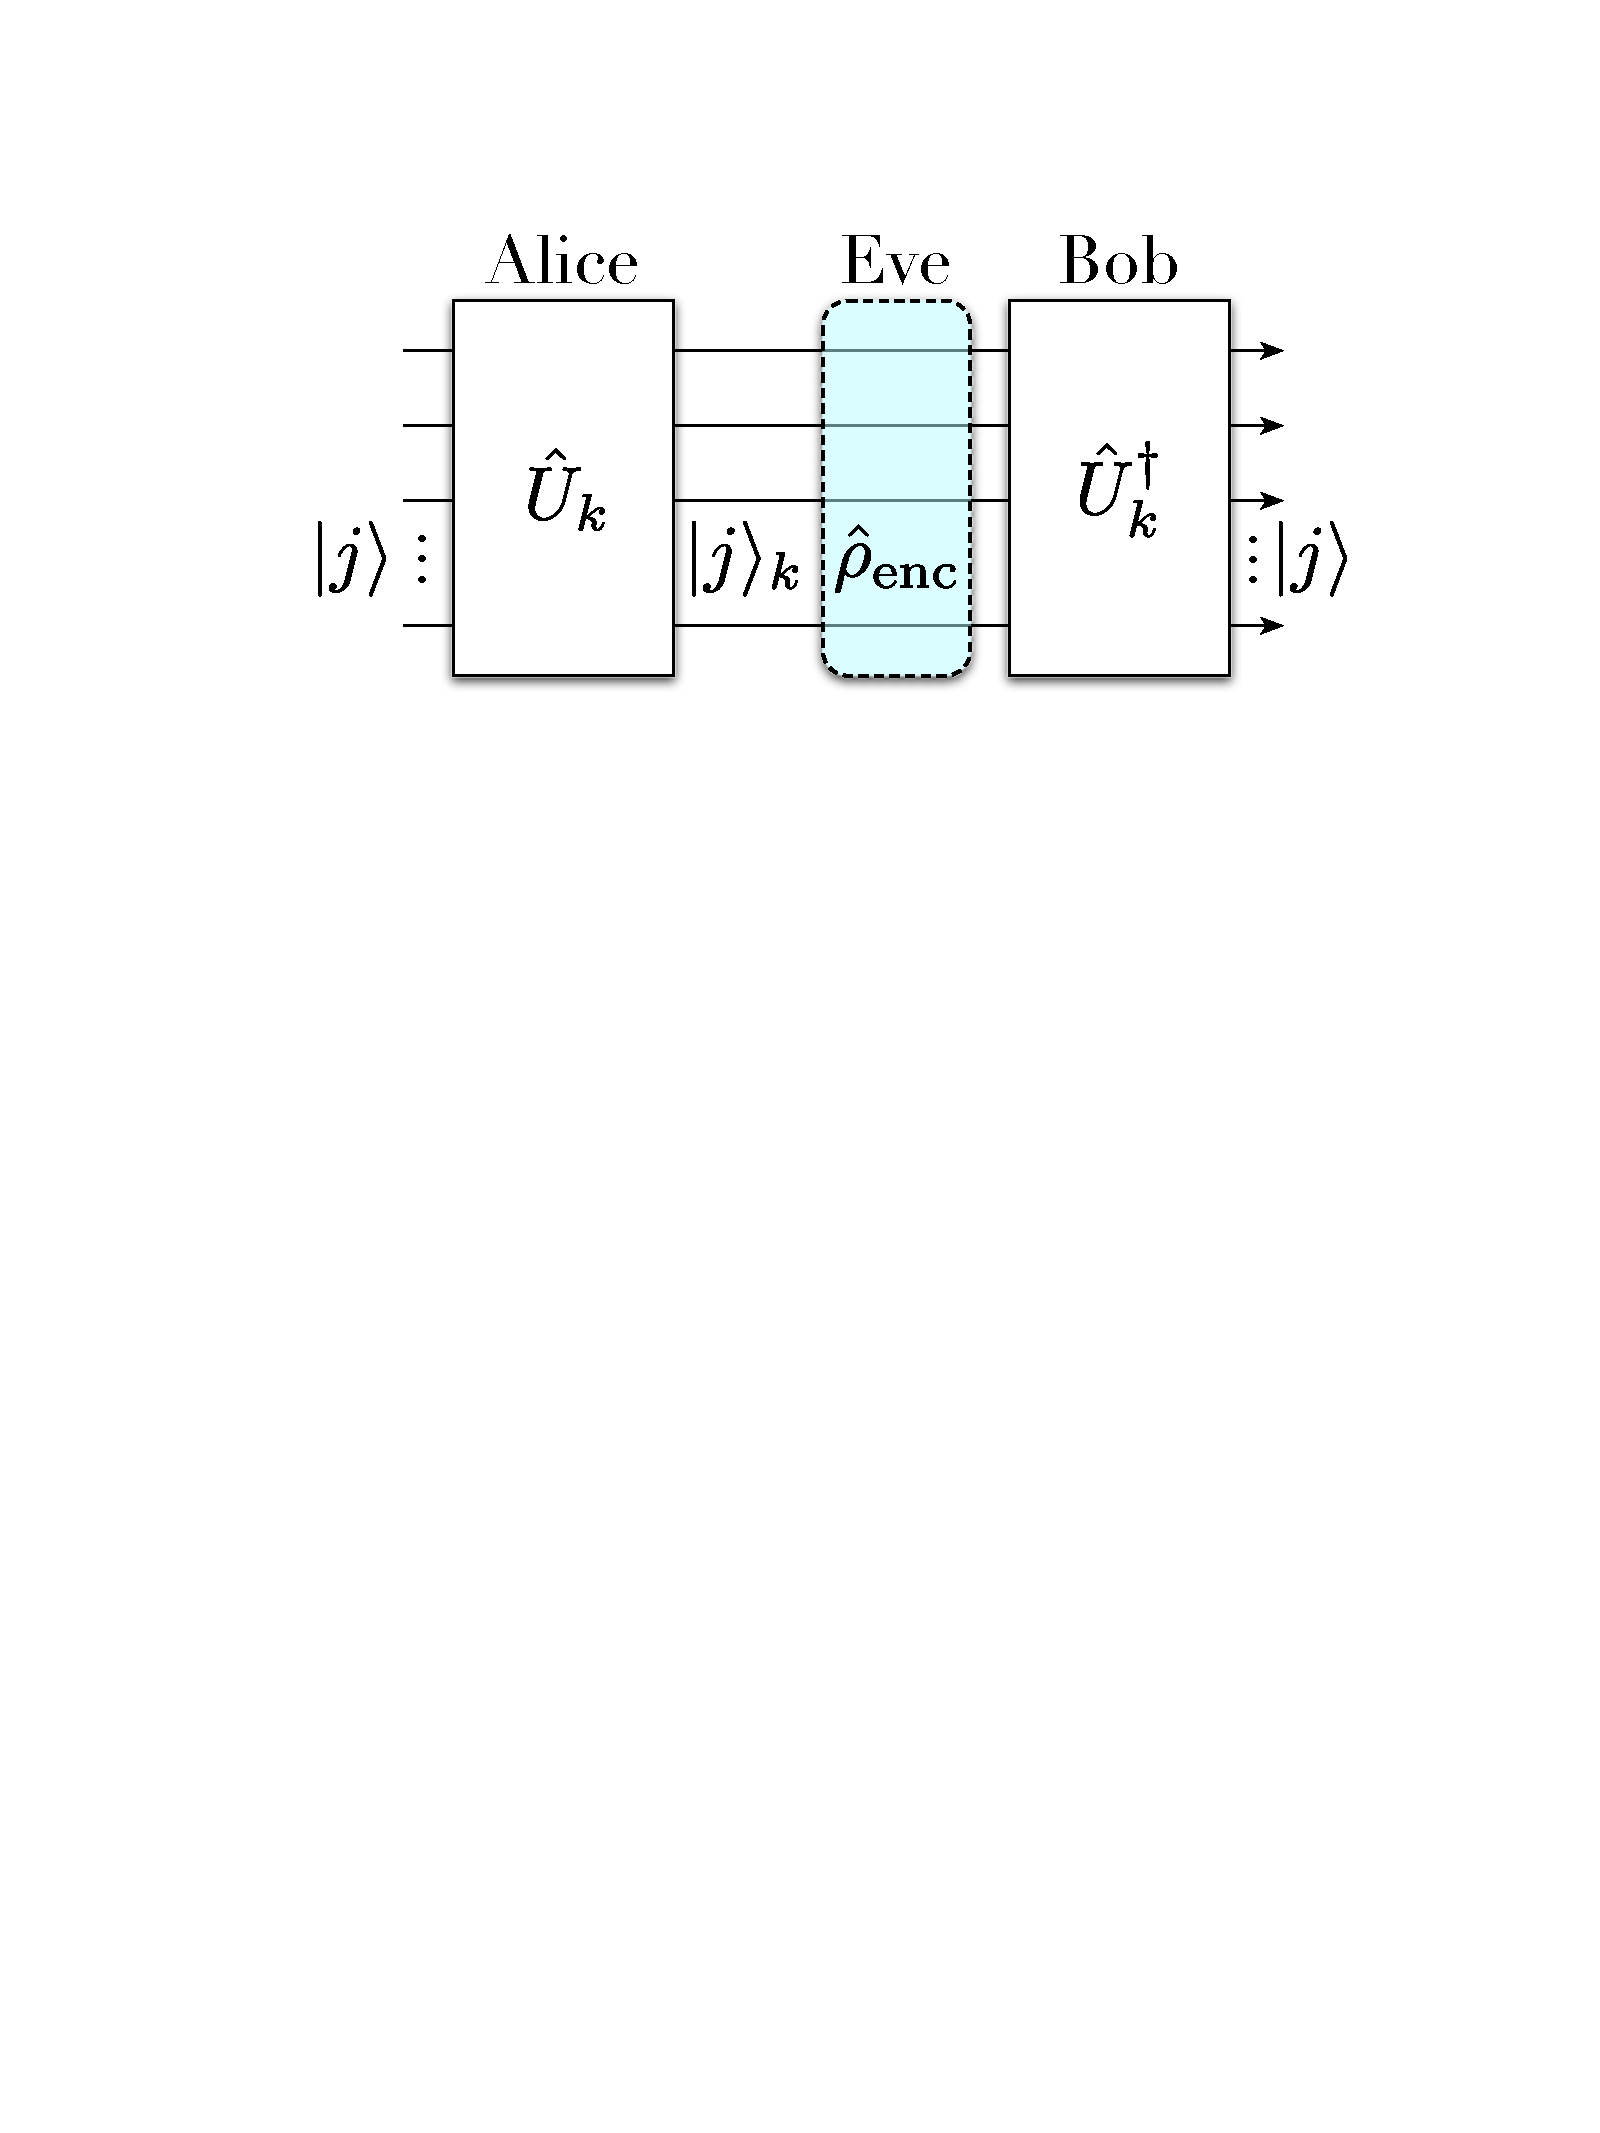
\includegraphics[width=0.475\textwidth]{enigma_machines}
\captionspacefig \caption{Schematic of the quantum Enigma machine protocol for quantum private-key cryptography. $\ket{j}$ is the message, $k$ is the key, and $\hat{U}_k$ is the encryption operation associated with key $k$, chosen randomly from the Haar measure. The encrypted message is $\ket{j}_k$. An eavesdropper intercepting the channel without knowledge of the key observes the state $\hat\rho_\mathrm{enc}$.}\index{Quantum Enigma machines}\label{fig:enigma}	
\end{figure}

Here Alice and Bob share a short secret key $k$ of length $m$, and wish to communicate a message $j$ of length $n$. The secret key might be established via conventional QKD. First off, they agree upon a set of Haar-random unitaries\index{Haar measure}, $\{\hat{U}_k\}$, associating one with each of the possible $2^m$ keys. This needn't be performed in secret. Alice then encodes her message into the state $\ket{j}$. Her encryption operation is to apply $\hat{U}_k$ to this state according to Alice and Bob's shared secret key, yielding the encoded state,
\begin{align}
\ket{j}_k=\hat{U}_k\ket{j},
\end{align}
which Bob is easily able to decrypt using the inverse unitary,
\begin{align}
\hat{U}_k^\dag\ket{j}_k=\ket{j}.
\end{align}

To characterise the security of the scheme, we first note that in the absence of knowing the key or message, and assuming all $j$ and $k$ are equally likely, Eve observes the mixed state,
\begin{align}
\hat\rho_\mathrm{enc} &= \frac{1}{2^{m+n}} \sum_{j,k} \hat{U}_k\ket{j}\bra{j}\hat{U}^\dag_k \nonumber\\
&= \frac{1}{2^{m+n}} \sum_{j,k} \ket{j}_k\bra{j}_k.
\end{align}
The security can now be quantified in terms of the accessible information\footnote{The accessible information is the maximum of the mutual information between Alice's input states and measurements performed on the encoded state by Eve.}\index{Accessible information} between this state and the plaintext state, which can be upper-bounded as,
\begin{align}
	I_c \leq n + \frac{1}{2^m}\max_{\ket\phi}\sum_{j,k} |\langle \phi|j\rangle_k|^2 \log |\langle \phi|j\rangle_k|^2.
\end{align}
It was shown that this quantity can be made arbitrarily small with key-size scaling as,
\begin{align}
m=O(\log n),
\end{align}
which represents very frugal requirements in key-size versus message length. They further showed that the scheme can be made robust against noise and loss.

Note that the security of the scheme is information-theoretic\index{Information-theoretic security}, and does not make any assumptions about computational security\index{Computational security}. Thus, this represents a strong form of quantum private-key cryptography, requiring only very short keys compared to message length.

However, the scheme is very challenging to implement on a large scale over long distances. Consider an optical implementation, where the message is photonically encoded. Now the scheme represents a complex, multi-mode, generalised Mach-Zehnder interferometer\index{Mach-Zehnder interferometer}, meaning that the channel between Alice and Bob, who might be far apart, must be interferometrically stabilised\index{Interferometric stability} (Sec.~\ref{sec:opt_stab}) on the order of the photons' wavelength (hundreds of nanometers for optical frequencies), which is extremely challenging over long distances.

%
% Hybrid Quantum/Classical Cryptography
%

\subsection{Hybrid quantum/classical cryptography}\index{Hybrid quantum/classical cryptography}

As discussed, the RSA public-key cryptosystem is vulnerable to an efficient quantum attack, whereas private-key schemes like AES\index{Advanced Encryption Standard (AES)} are not (believed to be). Thus, combining QKD schemes with private-key classical schemes does not compromise security in the quantum era.

Why would we combine quantum and classical encryption techniques when QKD is already provably secure, whereas the classical schemes are not?

In the near future, as QKD schemes begin their rollout in space and on Earth, random bits from the QKD implementation will be very expensive and exhibit low bandwidth. Suppose we wanted to securely videoconference across the globe. For just a single user this would require megabits per second of shared random bits, which will quickly saturate the capacity of overhead quantum satellites. Instead, let us use the QKD system to securely share just a 256-bit private session key\index{Session key} between two users. This is subsequently employed for AES256\index{Advanced Encryption Standard (AES)} encryption that operates entirely over the classical network, which we regard as extremely cheap. Importantly, unlike one-time pad implementations, this session key may be reused. Now we have a hybrid system which is not quantum-compromised, but which overcomes the cost and bandwidth issues associated with upcoming QKD networks.

While such a hybrid scheme is not information-theoretically secure (AES is not proven to be quantum-safe), the computational security assumptions are far stronger than for say RSA, since there are no known efficient quantum attacks against strong private-key schemes.

%
% Quantum Anonymous Broadcasting
%

\subsection{Quantum anonymous broadcasting} \label{sec:anon_broad} \index{Quantum anonymous broadcasting}

The previously described protocols all focussed on preserving the secrecy of messages. Alternately, it may not be the message that is sensitive, but rather the identity of the person who says it. \textit{Anonymous broadcasting}\index{Quantum anonymous broadcasting} is a protocol for achieving this.

Consider the following scenario. A group of users share a classical broadcast channel that anyone is able to transmit to, and everybody is able to listen to unencrypted. But it is of importance that the identity of whoever broadcasts to the channel must be kept secret from all users. \cite{Wehner} described a scheme for achieving this quantum mechanically using shared GHZ states -- \textit{quantum anonymous broadcasting} (QAB).

Let there be a (trusted) server that distributes GHZ states (of arbitrary numbers of qubits) to a group of users, one qubit per user. This can be prepared as described in, for example, Sec.~\ref{sec:GHZ_states}. Now if every user measures in the \mbox{$\ket\pm=\frac{1}{\sqrt{2}}(\ket{0}+\ket{1})$} basis the joint \textit{parity} (i.e whether an even or odd number of $+$'s were measured) is guaranteed to be even. For example, all users might measure $\ket{+}\bra{+}$, or exactly 2, but never exactly 1 or 3.

On the other hand, if a $\hat{Z}$ gate were applied to any one qubit, this would flip the parity outcome. Note that a GHZ transforms according to,
\begin{align}
	\hat{Z}_i \frac{1}{\sqrt{2}}(\ket{0}^{\otimes n} + \ket{1}^{\otimes n}) \to \frac{1}{\sqrt{2}}(\ket{0}^{\otimes n} - \ket{1}^{\otimes n})\,\,\forall \, i,
\end{align}
for any qubit $i$. This invariance in the location of the $\hat{Z}$ gate is the basis for the anonymity of the protocol. If a user wishes to broadcast `0' he does nothing, whereas if he wishes to broadcast `1' he applies the $\hat{Z}$ gate to his local qubit.

Finally, all users measure their qubits in the $\pm$-basis and publicly (without encryption) broadcast their measurement outcomes. All users now see all other users' measurement outcomes and are able to calculate the collective parity of the measurements. Now if the parity is even, the speaker must have said `0', whereas if it is odd he must have said `1'. The protocol is shown in Fig.~\ref{fig:QAB} and described in detail in Alg.~\ref{alg:QAB}.

\if 2\pubmode
\begin{figure}[!htbp]
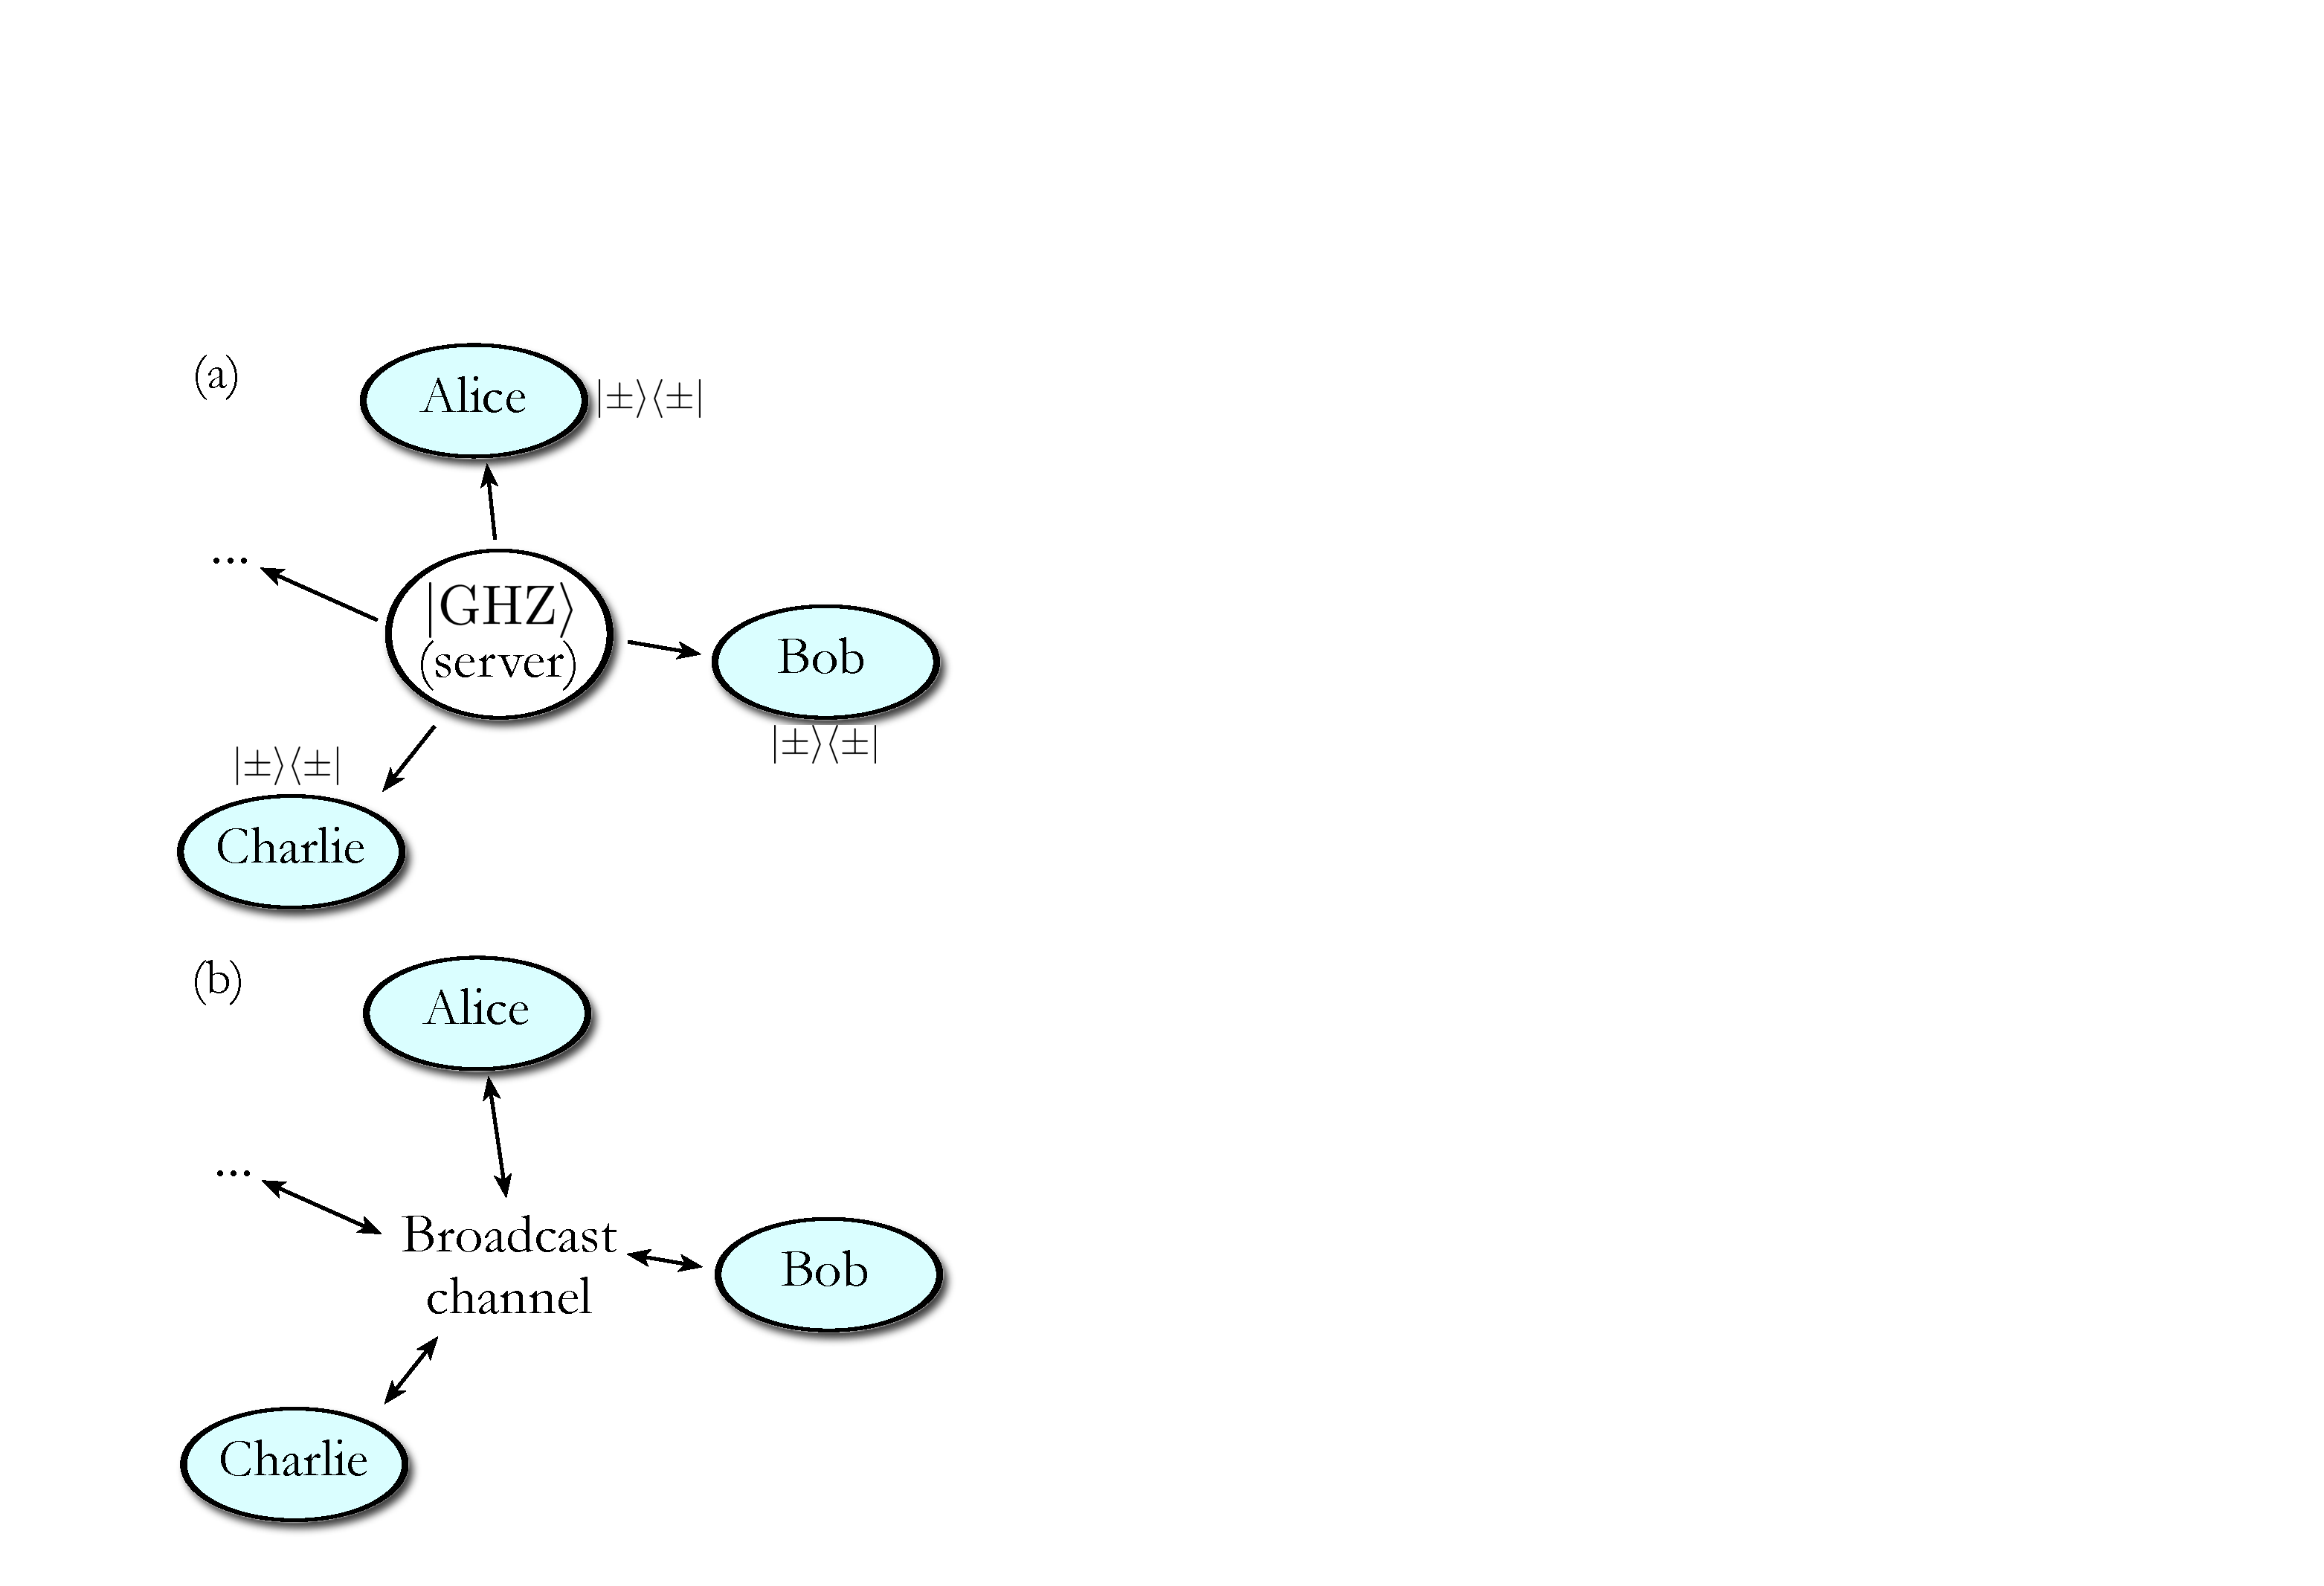
\includegraphics[width=0.475\textwidth]{QAB_long}
\captionspacefig \caption{Protocol for quantum anonymous broadcasting. (a) A central trusted server prepares GHZ states and distributes them amongst a group of users, one qubit per user. All users measure in the $\pm$-basis. (b) All users classically broadcast their measurement outcomes yielding shared random parity. During broadcast, the broadcaster lies about his measurement outcome to flip the joint parity if he wishes to transmit `1', or tells the truth to transmit `0'. The joint parity encodes the message of the anonymous user, which all listeners are able to recover. Importantly, only one user may broadcast at a time, otherwise the recovered message will be given by the XOR of all the simultaneously broadcast messages.} \label{fig:QAB}
\end{figure}
\else
\begin{figure*}[!htbp]
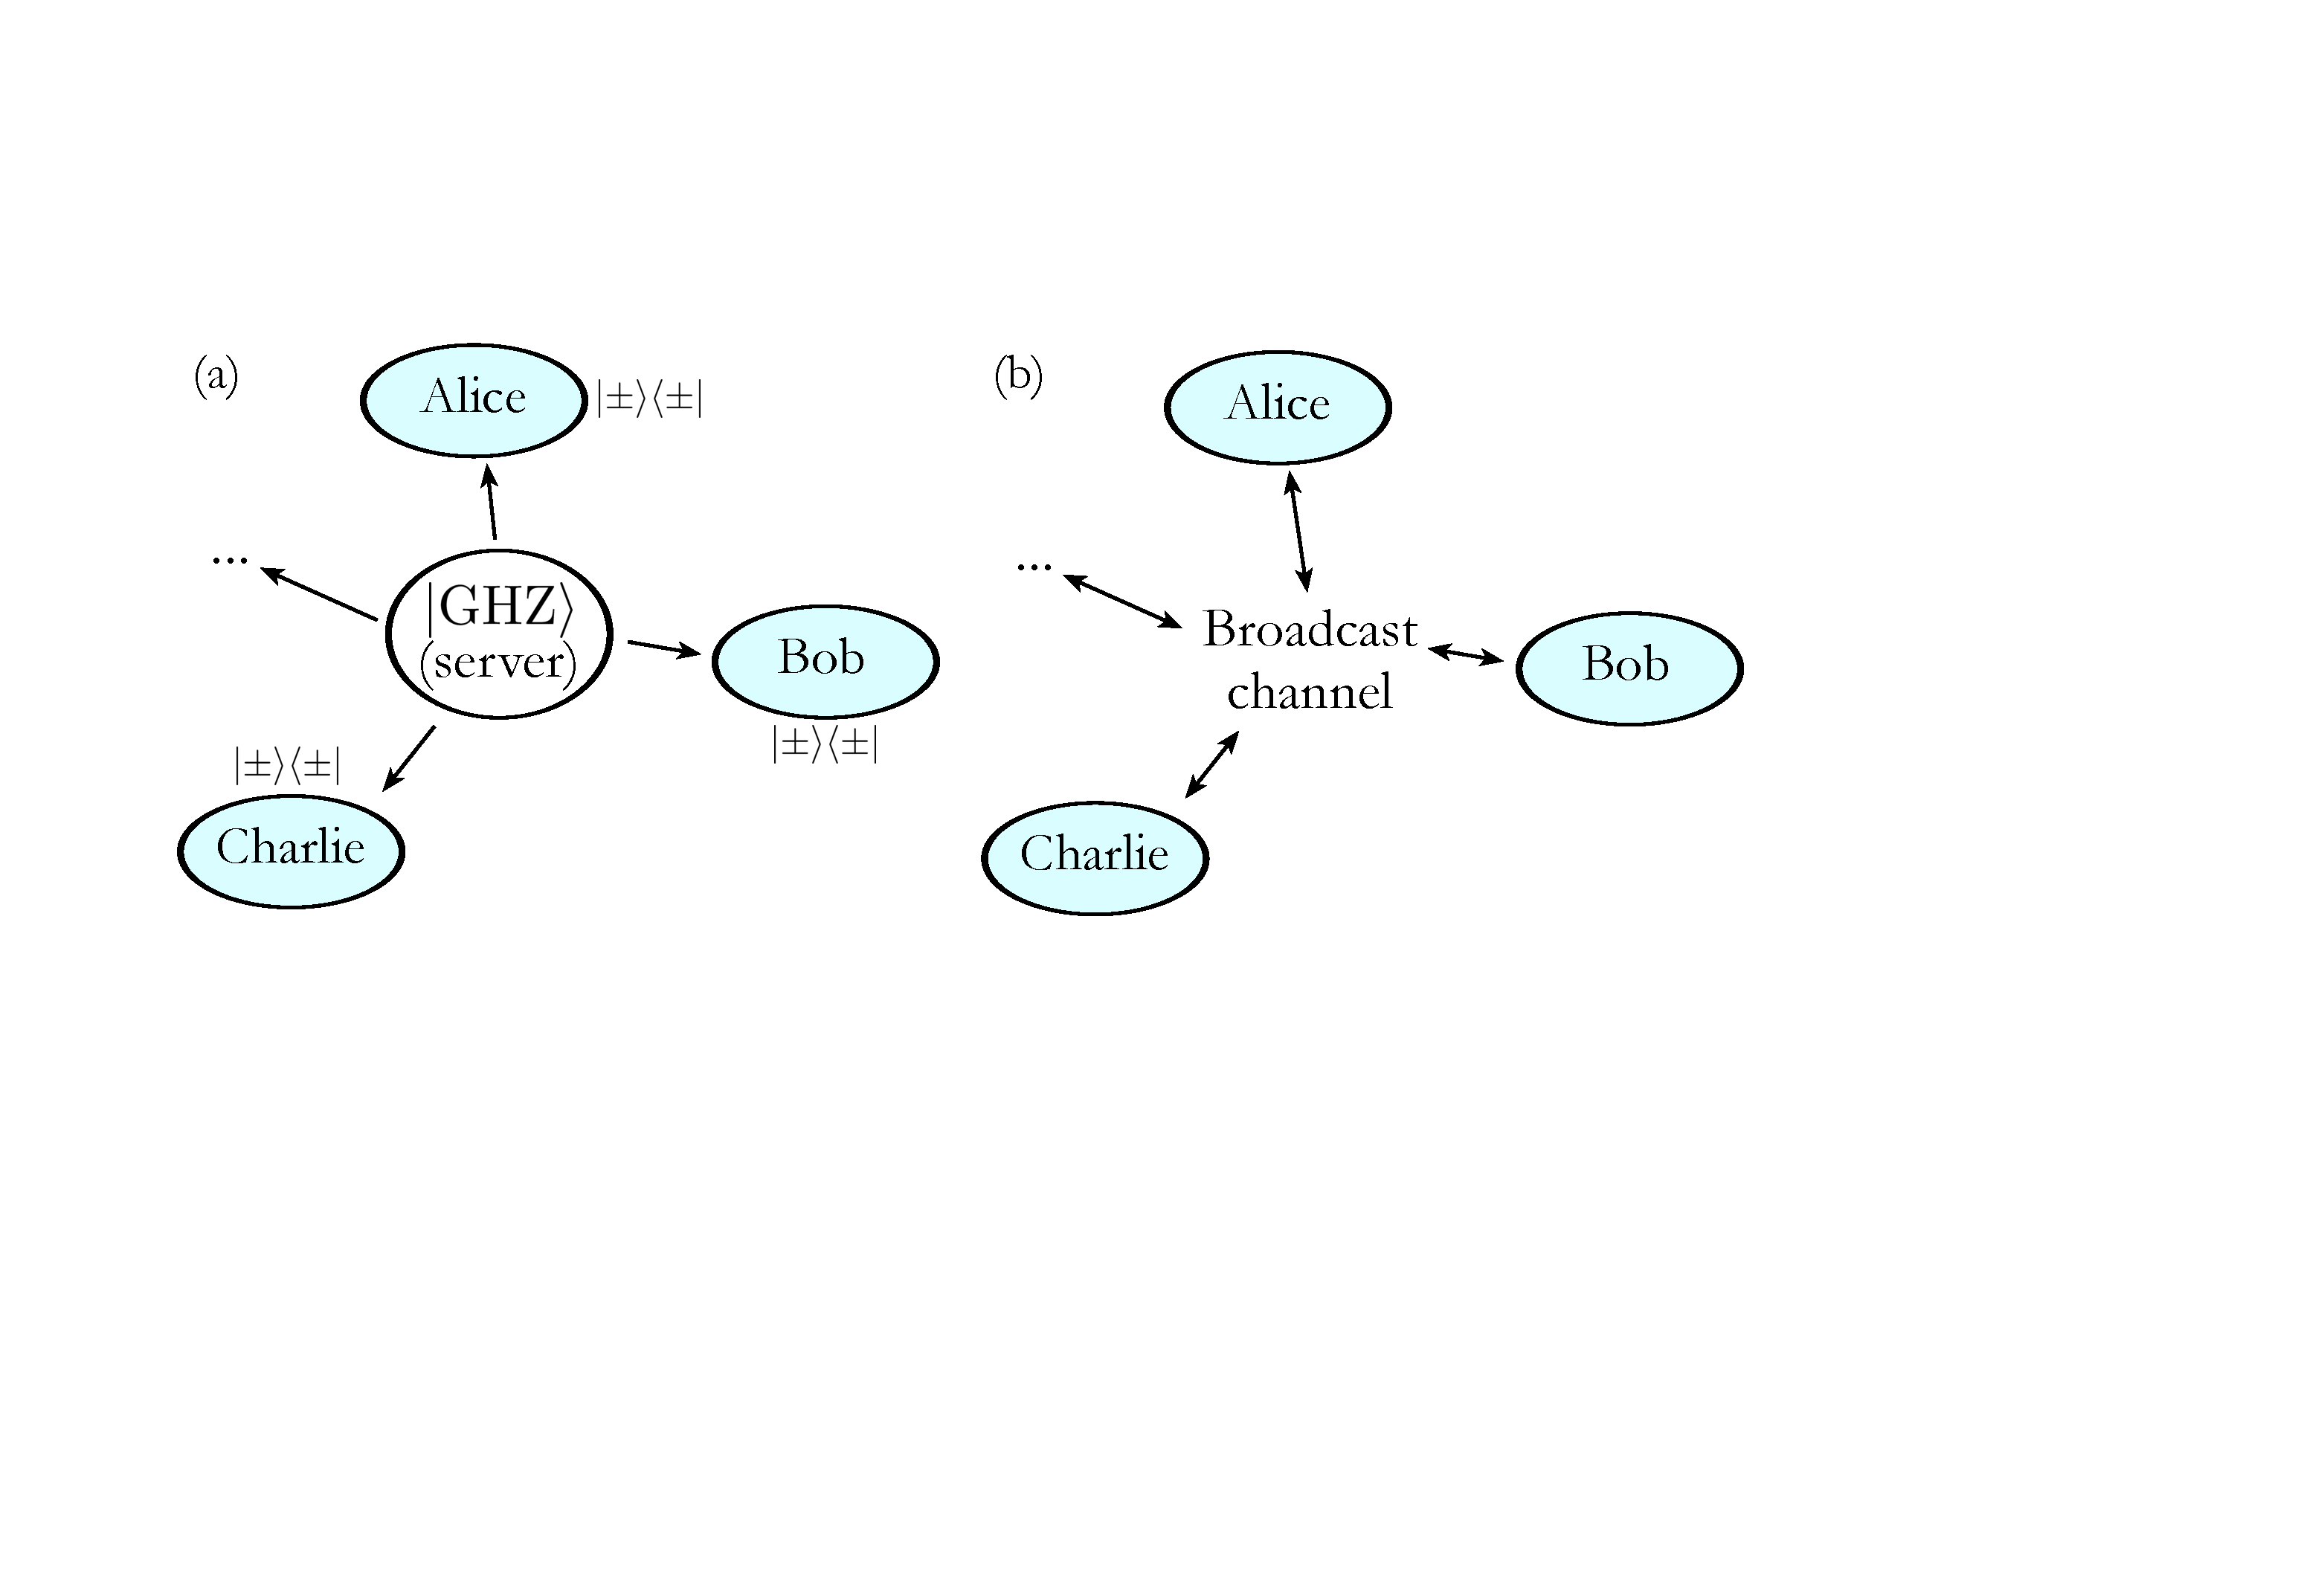
\includegraphics[width=0.8\textwidth]{QAB}
\captionspacefig \caption{Protocol for quantum anonymous broadcasting. (a) A central trusted server prepares GHZ states and distributes them amongst a group of users, one qubit per user. All users measure in the $\pm$-basis. (b) All users classically broadcast their measurement outcomes yielding shared random parity. During broadcast, the broadcaster lies about his measurement outcome to flip the joint parity if he wishes to transmit `1', or tells the truth to transmit `0'. The joint parity encodes the message of the anonymous user, which all listeners are able to recover. Importantly, only one user may broadcast at a time, otherwise the recovered message will be given by the XOR of all the simultaneously broadcast messages.} \label{fig:QAB}
\end{figure*}
\fi

\begin{table}[!htbp]
\begin{mdframed}[innertopmargin=3pt, innerbottommargin=3pt, nobreak]
\texttt{
function QuantumAnonymousBroadcasting(message, speaker):
\begin{enumerate}
\item $\ket\psi = \frac{1}{\sqrt{2}}(\ket{0}^{\otimes n}+\ket{1}^{\otimes n})$
\item $\ket\psi \to (\hat{Z}_\mathrm{speaker})^\mathrm{message}\ket\psi$
\item for(i$\in$users) \{
	\setlength{\itemindent}{.2in}
\item outcome$_i$ = measureInXBasis($\ket\psi_\mathrm{i}$)
\setlength{\itemindent}{0in}
\item \}
\item parity = $\sum_i$ outcome$_i$\,(mod\,2)
\item return(parity)
\item $\Box$
\end{enumerate}
}
\end{mdframed}
\captionspacealg \caption{Protocol for quantum anonymous broadcasting. The GHZ state is distributed in advance, one qubit per user. The measurement outcomes are classically broadcast without encryption. The final parity of the classical measurements reflects the message bit without identifying the speaker.} \label{alg:QAB}
\end{table}

Note that the scheme can be slightly simplified by rather than the speaker applying the $\hat{Z}$ to his qubit, upon announcing his measurement outcome he instead simply lies about his outcome and flips it. This follows simply because a $\hat{Z}$ gate prior to a $\pm$ measurement bit flips the classical measurement outcome, \mbox{$\hat{Z}\ket\pm=\ket\mp$}.

There are no constraints on time ordering of the measurements, nor, much like BB84, are there any interferometric requirements (not including the GHZ preparation stage), making this protocol very experimentally practical and robust over long distances.

Because of the time invariance in the measurements, distribution and measurement of the GHZ states can be performed well in advance of the actual message broadcast. This allows us to treat `shared parity'\index{Shared parity} as a fundamental resource (Sec.~\ref{sec:ent_ultimate}) for the QAB cryptoprotocol.

Since the parity-sharing can be isolated from the broadcasting stage it is unimportant if the GHZ source is non-deterministic or the channels for distributing it lossy. We can instead simply repeat GHZ distribution over and over at high repetition rate, post-selecting upon measurement outcomes where all users signal that they successfully received and measured their photons.

For these reasons, this scheme lends itself readily to photonic implementation, provided a reliable GHZ preparation circuit. The scheme has since been ported to operate on distributed toric codes\index{Toric code} to facilitate error correction of the distributed GHZ states \cite{bib:MenicucciExpQAB}.

%
% Quantum Voting
%

\subsection{Quantum voting}\index{Quantum voting}

The security of voting systems, and the anonymity of their voters are pressing issues in the modern world, and there have been countless high-profile instances of voting systems being compromised nefariously.

Based on similar ideas to quantum anonymous broadcasting is quantum voting, whereby a group of parties can anonymously vote such that no party, including the tallyman, is able to learn any individual voter's vote, but at the conclusion all are able to see the collective outcome of the vote.

There are a multitude of different models for voting, and a number of quantum implementations for them have been described. The two most well-known are:
\begin{itemize}
	\item Binary voting\index{Binary voting}: whereby each party votes `yes' or `no'. 
	\item Anonymous surveys\index{Anonymous surveys}: whereby each party votes a number and we wish to determine the sum of all the votes.
\end{itemize}

Fig.~\ref{fig:quantum_voting} and Alg.~\ref{alg:quantum_voting} describe a quantum implementation for anonymous surveys, using the protocol described by \cite{bib:VaccaroVoting}.

\begin{figure}[!htbp]
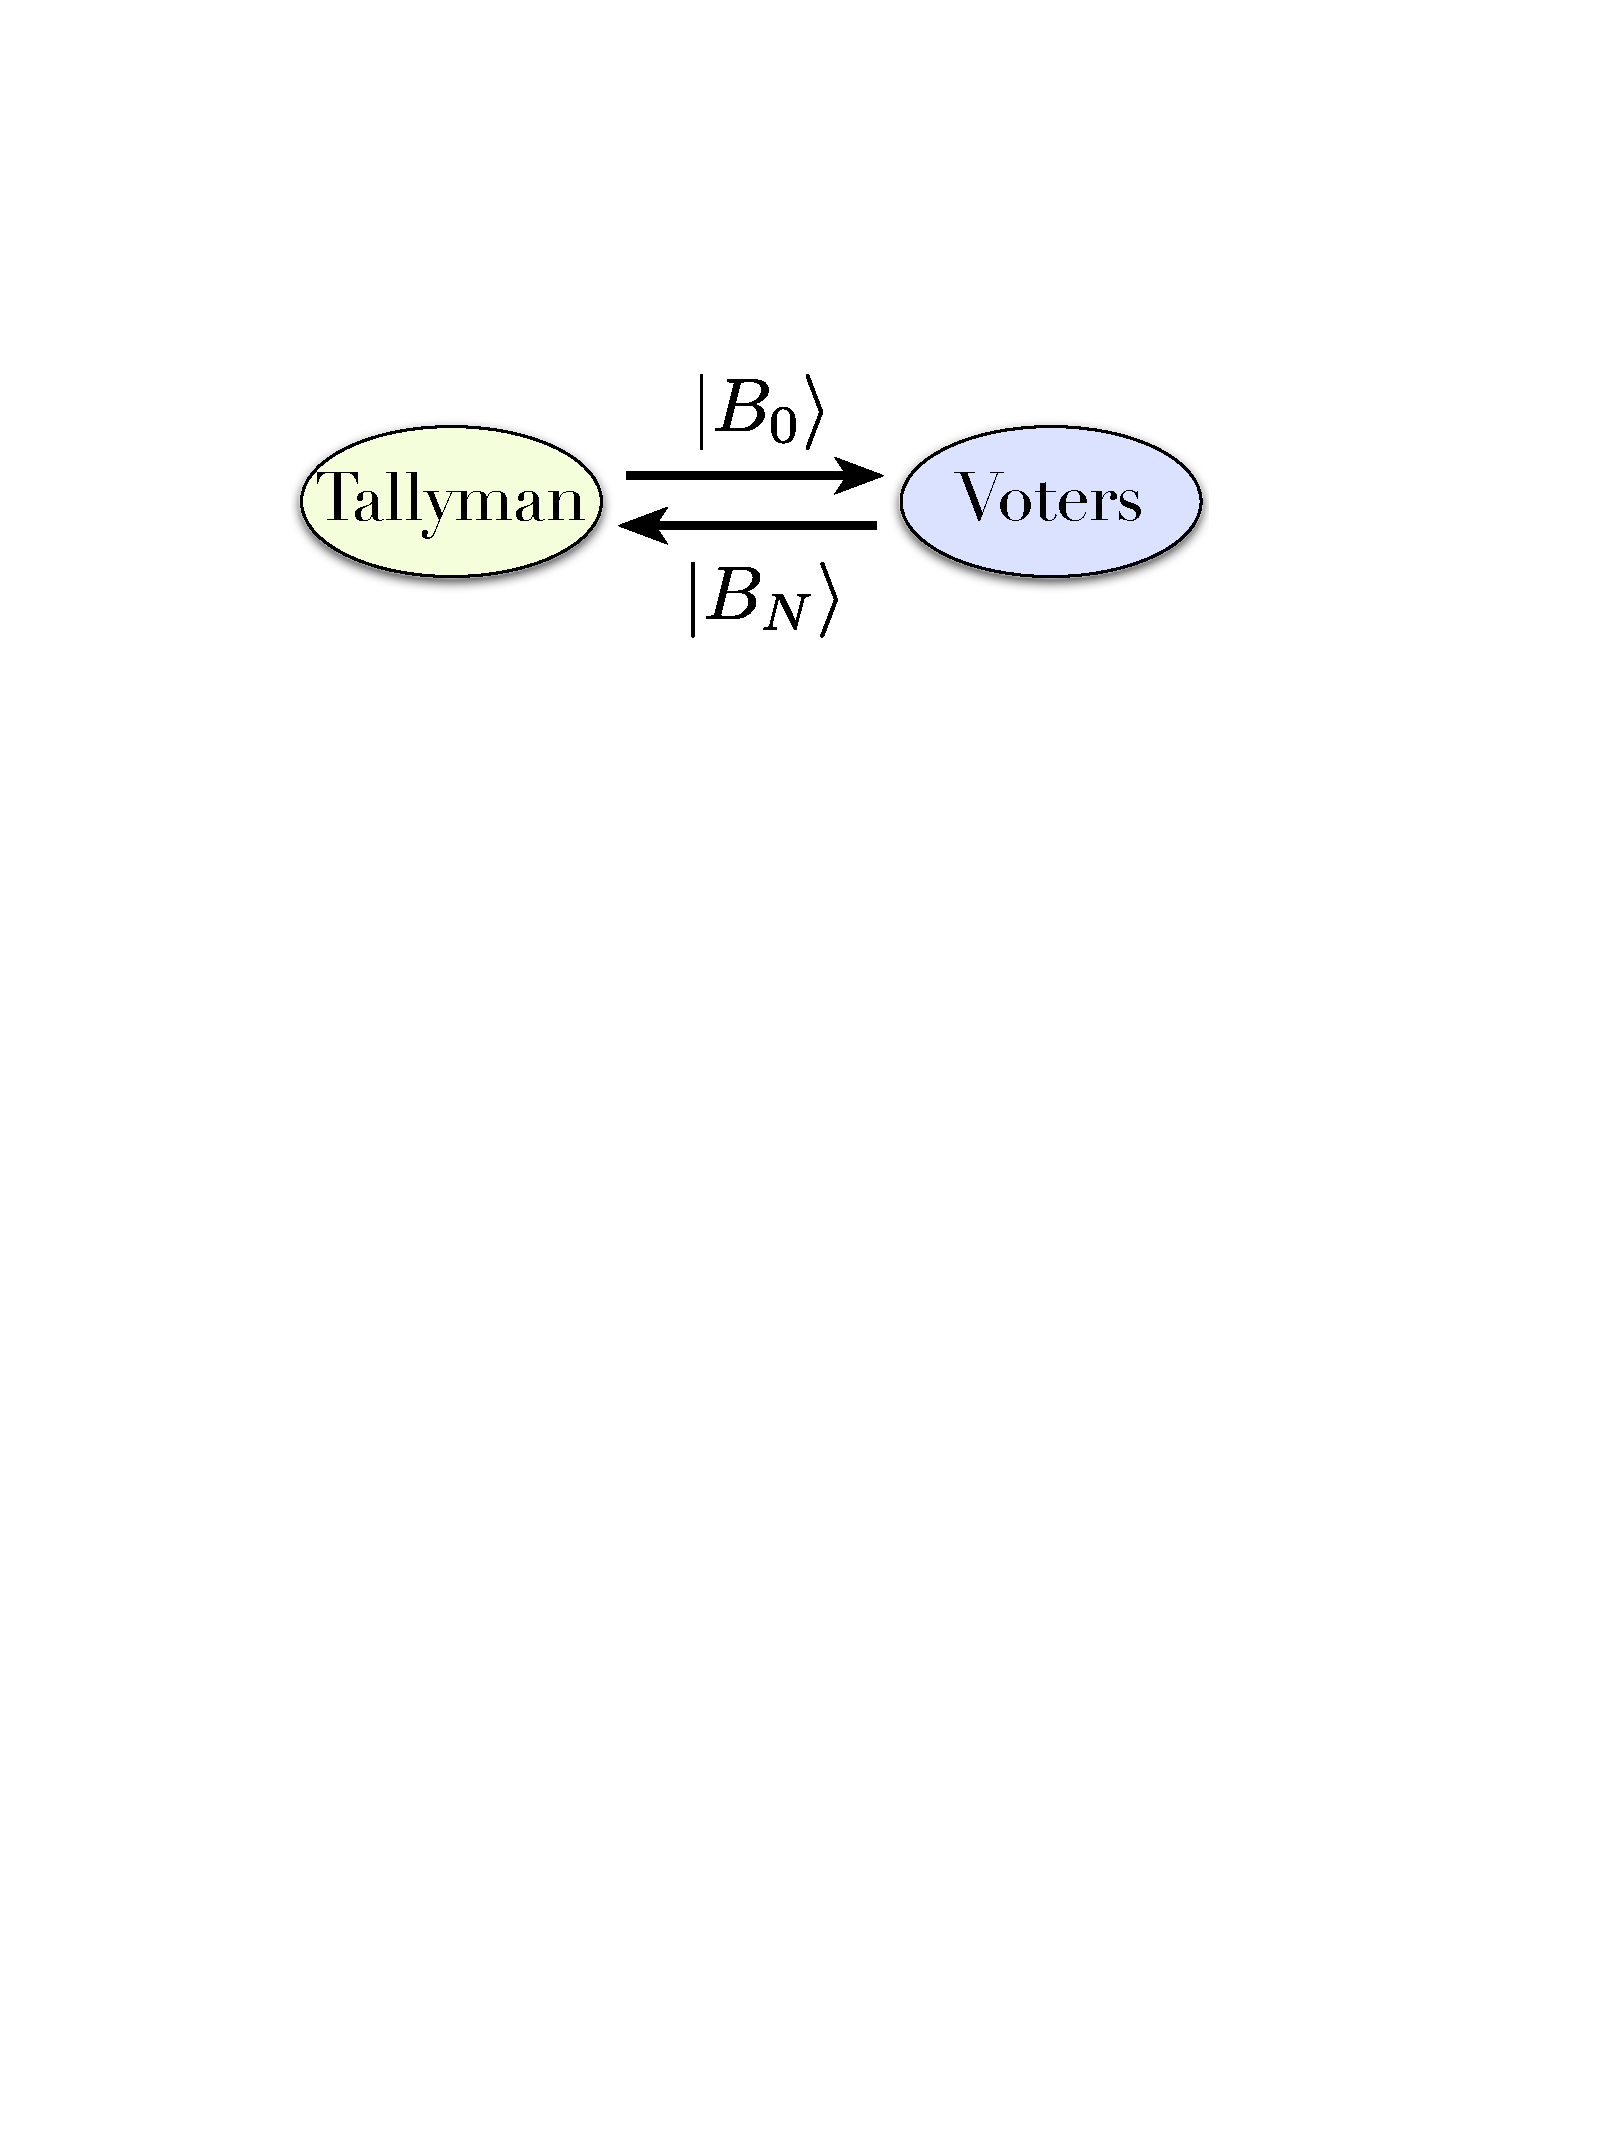
\includegraphics[width=0.35\textwidth]{quantum_voting}
\captionspacefig \caption{Protocol for quantum voting via anonymous surveying. The tallyman prepares the entangled state $\ket{B_0}$, half of which is shared with the votes. The voters each perform local phase-shift operations on the voters' half of the state, as per Alg.~\ref{alg:quantum_voting}. The phase-transformed state is then returned to the tallyman, who is able to extract the phase and hence the cumulative vote.}\label{fig:quantum_voting}\index{Quantum voting}	
\end{figure}

Conceptually, the scheme is similar to quantum anonymous broadcasting in that it hides votes in phases within an entangled state, which are not accessible to individual parties. The scheme relies on the preparation and distribution of a particular entangled state as a resource. Unfortunately this particular state is not one which is known how to be trivially prepared optically, and would therefore lend itself well to the outsourcing of preparation and distribution to a capable host via the quantum internet.

\begin{table}[!htbp]
\begin{mdframed}[innertopmargin=3pt, innerbottommargin=3pt, nobreak]
\texttt{
function QuantumVoting($\ket{B_0}$):
\begin{enumerate}
\item Prepare \textit{ballot state} for $N$ voters,
\begin{align}
\ket{B_0} = \frac{1}{\sqrt{N+1}}\sum_{n=0}^N \ket{N-n}_T\ket{n}_V,	
\end{align}
in the photon-number basis, where $T$ and $V$ represent the tallyman and the voters.
\item Each voter $j$ applies their vote operator,
\begin{align}
	\hat{v}_j = e^{i\pi\hat{n}_V \frac{\nu_j}{N+1}},
\end{align}
where $\hat{n}_V$ is the photon-number operator, and $\nu_j$ is the vote cast by $j$.
\item Following the $m$th vote,
\begin{align}
	\ket{B_m} = \frac{1}{\sqrt{N+1}}\sum_{n=0}^N e^{in\Delta_m} \ket{N-n}_T\ket{n}_V,
\end{align}
where,
\begin{align}
\Delta_m = \frac{2\pi}{N+1}\sum_{j=0}^m \nu_j,
\end{align}
is a scaled sum of the votes.
\item The state observed by the $T$ is,
\begin{align}
\mathrm{tr}_V(\ket{B_m}\bra{B_m}) = \frac{1}{N+1}\sum_{n=0}^N \ket{n}_T\bra{n}_T,	
\end{align}
which contains no voting information, similarly for $V$.
\item After all $N$ voters have voted, the voter state $V$ is transferred to the tallyman $T$.
\item Define the tally operator as,
\begin{align}
\hat{T} = \sum_{n=0}^N n\ket{T_n}\bra{T_n},	
\end{align}
where,
\begin{align}
\ket{T_n} = \frac{1}{\sqrt{N+1}}\sum_{j=0}^N e^{inj\frac{2\pi}{N+1}}\ket{N-j}\ket{j}.	
\end{align}
\item The tallyman finds the expectation value of the tally operator,
\begin{align}
r = \bra{B_N}\hat{T}\ket{B_N} = \sum_{j=0}^N \nu_j,
\end{align}
yielding the sum of all the votes.
\item return(r)
\item $\Box$
\end{enumerate}
}
\end{mdframed}
\captionspacealg \caption{Protocol for performing secure quantum anonymous surveying.} \label{alg:quantum_voting}\index{Quantum voting}
\end{table}

%
% Quantum Secret Sharing
%

\subsection{Quantum secret sharing}\index{Quantum secret sharing}

\comment{To do}

%
% Attacks On Quantum Cryptography
%

\section{Attacks on quantum cryptography}

\comment{To do}

Hacking attacks are related to the weaknesses of an implementation. A first common feature of hacking attacks is that they are feasible, or almost feasible, with present-day technology.

\subsection{Trojan horse attacks}

The best-known example is the family of Trojan horse attacks, in which Eve probes the settings of Alice’s and/or Bob’s devices by sending some light into them and collecting the reflected signal. 

Actually, the first kind of hacking attack that was considered is a form of Trojan horse that would come for free: it was noticed that some photon counters  silicon-based avalanche photodiodes  emit some light at various wavelengths when they detect a photon Kurtsiefer et al., 2001. If this light carries some information about which detector has fired, it must be prevented from propagating out, where Eve could detect it. 

\subsection{Quantum side channel attacks}

\subsection{Photon-number splitting attacks}

\cite{PhysRevLett.68.3121}

A beam-splitting (BS) attack translates the fact that the light that is lost in the channel must be given to Eve: specifically, Eve could be simulating the losses by putting a beam splitter just outside Alice’s laboratory, and then forwarding the remaining photons to Bob on a lossless line. The BS attack does not modify the optical mode that Bob receives: it is therefore always possible for lossy channels and does not introduce any error.

When the signal can consist of more than one photon, Eve can count the number of photons in each signal and act differently according to the result n of this measurement. Such attacks are called photon-number splitting PNS attacks
% \comment{Attacks based on bad implementation rather than bad theory}

PNS were discovered as zero-error attacks against BB84 implemented with weak laser pulses; in the typical parameter regime of QKD, even the Poissonian photon-number distribution can be preserved  Lu{\" u}tkenhaus and Jahma, 2002, so that the PNS attack cannot be detected even in principle as long as one known signal intensity is used. Use of different intensities in order to detect PNS attacks is the idea behind the decoy-states method. The distributed-phase-reference protocols also detect PNS attacks.